% !TeX root = main.tex
\chapter{Background}\label{chp:background}

\section{Fundamentals}

% Sound is linear - has a beginning and an end, constrained by the arrow of time
% Cannot be searched or skimmed
% Sound is one-dimensional
% We never stop listening
% Huge range of frequencies and pressure levels

%Audio is an electronic representation of sound which stores pressure waves as an electrical signal.

\subsection{Sound}
% Characteristics of sound
One of the distinuishing characters of radio is that it is based exclusively on sound.
Sound is defined as vibrations that travel through a medium, typically air, which humans perceive through their ears.
As it is based on vibration, sound cannot exist in a moment -- it can only take place over a period of time.
Sound is linear, as it is based on a sequence of motion.
It is experienced at a consistent rate, which cannot naturally be increased or desreased.

% challenges of sound
This time-based nature of sound gives it a fascinating character.
However, the time-based nature of sound comes with a variety of challenges.
Sound cannot be experienced instantanously, as it is the change in air pressure which produces sound.
As such, it takes time to consume sound.
For consuming long sound recordings, this property means that listening requires an investment of time.
In radio production, much of the time required to produce a programme must be committed to listening to the sound that has been recorded.
%The purpose of listening to the sound includes a variety of reasons, including reminding themselves of what
%was said, working out whether the sound quality is acceptable, deciding which bits of the recording to use, and many
%more.

To overcome the challenges that come with the temporal nature of sound, there are a number of technological solutions
that can be applied. At the very simplest level, sound can be navigated using rewind and fast-forward, to allow
listeners to re-listen or skip ahead to a sound recording. The playback rate of sound recordings can also be increased,
but there are limitations to this, which we discuss in Section X. However, in order to navigate sound with purpose, it
is preferable to be able to understand what is contained within the sound, and to be able to comprehend this
information efficiently. There have been two main approaches to achieving this -- audio visualization and semantic
audio analysis.

%From Dhanesha2010:
%It is a common practice for us to skim textual content on a web page. While skimming, we usually skip words or phrases
%that are not of interest to us and we slow down our speed when the content seems to be of relevance to us. But when we
%listen to audio content, which is not persistent and is sequential, such skimming is not possible.

Audio visualization attempts to take advantage of the properties of the human visual system by mapping sound to images.
This is done to allow listeners to see the sound in a way they can understand and make use of. This approach takes
advantage of the spatial layout that is possible with images, and the natural searching and skimming capabilities of
the human visual system.

Semantic audio analysis refers to a collection of techniques for analysing sound signals to extract human-readable
information from them. This can be used to map sound to high-level information, such as the name of the person
speaking, or the text of what they are saying. These techniques can vary from low-level features such as the most
dominant frequency, to high-level features such as the text of the words that are being spoken. These techniques can
also be combined with visualization methods to display the results.

As part of this work, we want
to understand how these techniques can best be applied to the production of radio, and make the process more efficient
by reducing the time that is needed to produce the programme. 

\subsection{Audio visualization}

Vision is very different medium that varies not only over time, but over space. When you remove the element of time,
you are left with an image that can be experienced instantanously, searched and skimmed.  Human vision can be used to
process complex scenes at a glance
%Anderson 2009; Belopolsky et al. 2008; Goldstein 2010
For this reason, visualisation is a good way to interact with time-variant information.  \citet{Aigner2011} contains a
collection of examples of how this can be done.

Visual systems can be used to complement audio interfaces, as they are able to address the key challenges of sound.

In modern society, screens for displaying visual content are widely available.

Sonic Visualiser from \citet{Cannam2010} can be used to generate these visualisations.

To be able to represent audio visually, we must map auditory properties to visual properties. We could select these 
to have a general mapping, which attempts to cover all use cases, or a selective mapping that targets a particular use
case.

When attempting to link sound and vision, it is desirable to create a mapping that is coherent and makes sense to the
user. The ultimate goal would be to create an audio visualisation that ``look likes it sounds'', as this would
allow users to comprehend the sound without having to listen to it.

%In a world of `big data', data visualization is becoming an increasing popular subject. Visualization techniques have
%been applied to audio content for a
%variety of applications including accessibility \citep{Ho-Ching2003}, browsing
%large databases \citep{FontCorbera2010}, browsing small databases \citep{Yoo2011} and musical training
%\citep{Ferguson2005} amonst others.

%The development of good visualizations lies somewhere between science and art.
%Tufte's seminal work on good practice \citep{Tufte2001} gives solid guidance on
%creating elegent and unbiased visuals, and Wolfe and Horowitz \citep{Wolfe2004}
%tell us which properties of vision are most critical for visual search.
%However, putting these together in the context of audio requires a certain
%amount of creativity.

%This project focusses on `visualization of time-oriented data', a good overview
%of which can be found in a Springer book of the same name \citep{Aigner2011}.
%The rest of this section will look at examples of time-oriented visualization
%of audio, grouped by the most common visualization techniques.

\subsubsection{Crossmodality}
Crossmodal perception is a term used to describe interaction between the different senses. This phenomenon has been
studied over many years by psychologists, who have discovered perceptual mappings between auditory and visual stimuli.

The ``bouba/kiki effect'' is a demonstration of cross-model mapping between vision and audition, originally discovered
in an experiment run by psychologist \citet{Koehler1929}. In the experiment, participants are shown two abstract shapes
and are asked to assign the name `bouba' to one of them, and `kiki' to the other \footnote{K\"ohler used the words
  `baluma' and `takete' in the original experiment, but the result was the same.}. To try out the experiment for
yourself, without reading ahead look at the shapes in Figure~\ref{fig:boubakiki} and see which shape you think best
fits the name `bouba' and which best fits `kiki'.


\begin{figure}[ht]
\centering
  \centering
  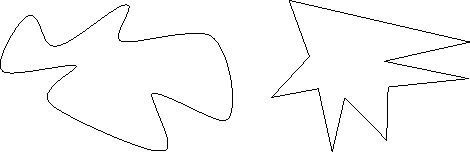
\includegraphics[width=0.8\linewidth]{figs/bouba-kiki.pdf}
  \caption{Demonstration of the ``bouba/kiki effect'' \citep{Ramachandran2001}}
  \label{fig:boubakiki}
\end{figure}

K\"{o}hler found that the vast majority of participants chose to name the sharp, pointy shape `kiki' and the curvy,
rounded shape `bouba'. \citet{Ramachandran2001} found that that this effect holds for 95--98\% of the population. This
is an example of just one audio-visual mapping that is common amongst the population.

\citep{Hubbard1996} did some work to determine which sounds related to which visual properties

%These audio-visual associations are not just higher-level constructs that our
%concious brain creates, they affect the brain at the very lowest level even
%with only brief exposure to bimodal stimuli. Zangenehpour et. al.
%\citep{Zangenehpour2010} used a PET-CT scanner to measure blood flow in the
%brain during exposure to audio and visual stimuli. ``When presented with only
%the auditory or visual components of the bimodal stimuli, na\"{i}ve subjects
%showed only modality-specific cortical activation, as expected.  However,
%subjects who had previously been exposed to the audiovisual stimuli showed
%increased cerebral blood flow in the primary visual cortex when presented with
%sounds alone.''

\citet{Spence2011} reviewed a wide range of psychology experiments that attempt to find the inherint cross-modal links
in the human brain, including audio-visual mapping.  There are two common types of test methods used to discover these
links -- `speeded' and `unspeeded'.  In `speeded' tests, participants are tasked with classifying an audio/visual
stimulus and their reaction time is measured. When the auditory and visual stimuli are `congruent' (perceived to be
similar), then their reaction times are quicker. In `unspeeded' tests, visual and audio stimuli are presented very
quickly, one after the other, and participants are asked to select which stimulus came second. When the stimuli are
congruent, participants find it more difficult to work out the order of presentation.
Through his literature review, \citet{Spence2011} found there to be strong evidence for six audio-visual mappings,
which he grouped into three categories, shown in Table~\ref{tab:crossmodal}.

\begin{table}
\centering
\begin{tabular}{|l|l|l|}
\hline
\textbf{Type} & \textbf{Link} & \textbf{Direction} \\ \hline
Structural    & Loudness/brightness  & louder=brighter \\ \hline
\multirow{3}{*}{Statistical} & Pitch/elevation & higher=higher \\ \cline{2-3}
              & Pitch/size & higher=smaller \\ \cline{2-3}
              & Loudness/size & louder=bigger \\ \hline
\multirow{2}{*}{Semantic} & Pitch/elevation & higher=higher \\ \cline{2-3}
              & Pitch/spatial frequency & higher=higher \\ \hline
\end{tabular}
\caption{Audio-visual mappings supported by strong evidence \citep{Spence2011}}
\label{tab:crossmodal}
\end{table}

\citet{Tsiros2014} used a different approach to measure audio-visual crossmodality by using audio visualization
techniques.  Three audio recordings were used -- a violin, recording of wind noise and impact sound event. For each,
images were manually created which used different combinations of audio-visual mappings (e.g. dissonance $\to$ texture
granularity). Participants were played an audio clip and shown an image and were asked whether they are similar or not,
and to what degree (on a scale of 0--100).  The experiment confirmed previous results which found strong links between
size/loudness and pitch/elevation, and weaker links between colour/pitch, granularity/dissonance, and colour
complexity/dissonance.
%Tsiros confirms the results revealed by previous studies [7], [15], [19] which found strong relationships between the
%audio-visual feature associations of size – loudness, pitch – vertical position, and weaker relationships between
%color – pitch, texture granularity – sound dissonance and color complexity- sound dissonance

Additional work from \citet{Marks2003} suggests that cross-modal interaction is a result of late-stage cognitive
processes.

Artwork that used synaesthesic style mapping for music to colour \citep{Armitage2012}

Relationship between pitch and colour \citep{Datteri2004}

Cross-modality can even be measured in the visual cortex using a PET scanner \citep{Zangenehpour2010}

%Vision and audition are physiologically separate, but idential in many respects
%\citep{Tsiros2013}.

In this section, we have seen that the temporal constraints of audio can be overcome by using the spatial properties of
vision. These mappings can be designed to be general, or address specific tasks. There are underlying links between
sound and vision that could be exploited to make more perceptually relevant visualisations.

\subsection{Waveforms}

An audio waveform is the graphical representation of an audio signal. It is perhaps the simplest audio visualisation
technique available and arguably the most commonly used.

Audio waveforms have been used to visually representing audio content ever since the first digital audio workstations
started to appear \citep{Massie1985}. Despite their ubiquity, they display very little relevant information and are not
well-suited towards most audio navigation or editing tasks. For instance, it is almost impossible to distinguish
between individual voices with a waveform, even if they sound very different.

% ==== PROS ====

The curve of an audio waveform directly represents the pressure waves of the sound, so the amplitude and frequency of
the sound is mapped to the amplitude and frequency of the plot. This makes it conceptually easy for users to
understand how the audio is represented.

Large curves represent loud sounds, and spatially high frequency curves represent high sound frequencies. These
mappings corrolate with two of the most common cross-modal links (see Table~\ref{tab:crossmodal}).

Waveforms operate in the time domain and can be plotted using a linear function of the audio signal, which makes them
computationally efficient to generate. 

For these reasons, it is the default audio visualisation used in all audio editing software that we have come across.

% ==== CONS ====

In waveforms, frequencies are visible (see Figure~\ref{fig:waveform-zoomin}) at the right scale, but it is hard to work
out which exactly which frequencies are present and in what proportion.

Given a high enough resolution, waveforms can be losslessly be converted back into the original audio signal. In this
sense, they can fully represent the information contained in the audio. However for any practical application, the
time axis of the waveform must be downsampled so that the waveform can be viewed at a reasonable scale (see
Figure~\ref{fig:waveforms}).  This downsampling causes the frequency informaton to be lost, and what remains is the
profile of the audio amplitude.

``Graphically displaying an audio recording as a waveform would generally be inappropriate because, for most users, the
audio signal spectrum offers no information about content'' \citep{Bouamrane2007}.

\begin{figure}[p]
  \centering
  \begin{subfigure}{.5\textwidth}
    \centering
    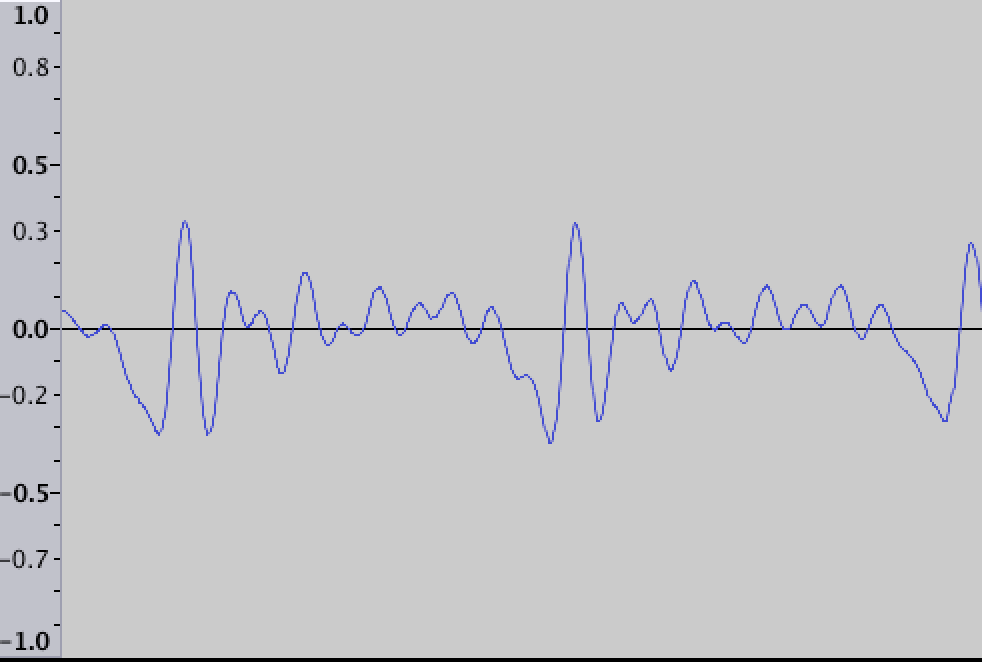
\includegraphics[width=.9\linewidth]{figs/waveform-zoomin.png}
    \caption{When zoomed-in, the frequency information is visible}
    \label{fig:waveform-zoomin}
  \end{subfigure}%
  \begin{subfigure}{.5\textwidth}
    \centering
    
\includegraphics[width=.9\linewidth]{figs/waveform-zoomout.png}
    \caption{When zoomed-out, the frequency information is lost and only the amplitude profile is visible}
    \label{fig:waveform-zoomout}
  \end{subfigure}
  \caption{The effect of scaling on waveform frequency information}
  \label{fig:waveforms}
\end{figure}

This amplitude profile can be used to infer some information about the audio content. For example, speech content has
frequent short periods of silence between words, whereas music has few periods of silence. However, in order to be able
to read this information, users must learn what the different profiles of sounds look like.

Many professional engineers and producers have worked with waveforms for most of their career, and have developed the
skills to be able to read waveforms.  However, without frequency content, there is a limit to the amount of information
waveforms can convey.

We searched for studies that considered the performance of waveforms as an interface to audio content. Although X and Y
included waveforms in their studies, the waveforms themselves were not assessed. No studies could be found that
consider the performance of the waveform itself.

\subsection{Spectrograms}
The spectrogram is a visual representation of the spectrum of frequencies in an audio signal over time.  This technique
allows the full frequency content of the audio to be visible to the user. It is a simple mapping that can be easily
understood, and a generic visualisation that can be used for a wide variety of applications.

Unlike waveforms, spectrograms make it easy for the user to see the frequencies that make up the sound, and in what
proportions. When the time axis of spectrograms is rescaled, the frequency information is still visible, so it is much
more robust to scaling than waveforms. This allows a higher density of information at typically-used scales.

The frequency scale in an audio spectrogram is usually presented on a logarithmic or Mel scale to give a better mapping
of frequencies to the perception of pitch. Psuedocolour (see Section~\ref{sec:pseudocolour}) is often used so that the
detail is more visible.

Higher audio frequencies are displayed at the top of the spectrogram, and the energy of the signal is mapped to the
intensity of the colour. Like with waveforms, these corrolate to two of the cross-modal links listed in
Table~\ref{tab:crossmodal}.

Spectrograms are available in most audio editing software, but rarely used by default. As spectrograms are based on a
Fourier analysis, they are more computationally expensive to plot than waveforms, but trivial for modern computers to
generate.

Although spectrograms present the data very clearly, users must still learn how to interpret the information.  
\citet{Zue1986} found that expert users were able to use spectrograms to read the phonemes of speech, but this is
impossible for the average user to achieve.

The spectrogram displays the energy present in each frequency band, however this can make it difficult for the user to
see the overall energy at a given time.

Spectrograms have a wide range of parameters which control how the data is displayed, including window size and 
shape, frequency and energy scaling, min/max values and pseudocolour methods. This means that is a great deal of
inconsistency between spectrogram, which can make it difficult for users to move from one to the other.

Understanding spectrograms requires users to have basic knowledge about how audio is composed of multiple frequencies.
They would also benefit from understanding how frequencies interact, such as harmonics.

Can be used to edit frequencies like photoshop \cite{Boogaart2006}

%Pros
%X info rich
%X robust to scaling
%X already available
%X simple and generic visualisation
%X computatonally easy

%Cons
%X more computationally expensive than waveforms
%X must learn what different things look like - hard to map frequencies to info
%(doesn't take into account octaves and harmonics)
%X total energy is unclear
%X users must understand that audio is composed of a spectrum of frequencies
%X multiple parameters needed to control visualisation - inconsistent (e.g. window size, window type, 

Spectrograms provide an information-rich and scalable alternative to waveforms, and they are widely available in most
audio editing software. Despite this, waveforms remain a more popular way of interacting with audio. It is unclear as
to why this is.

\subsection{Semantic audio}
Semantic audio is the extraction of perceptual attributes from an audio signal, which is used to describe sound in
human-readable terms.

% What is semantic audio?
describe sound in human-readable terms
decomposing acoustic signals into semantic entities
can be applied to semantic user interfaces
extracting and describing the perceptual attributes of sound

classification

Review of audio information retrieval \citep{Foote1999}, including automatic speech recognition, word spotting, speaker
and music identification, and audio similarity

% classification/tagging
This paper divides audio streams into five classes: silence, noise, pure speech, speech over background sound and
music. Four new features are proposed, including silence ratio, pitch frequency standard deviation, harmonicity ratio
and smooth pitch ratio. \citep{Liang2005}
Survey \citep{Duan2014}

% speech-music discrimination
Comparison of features \citep{Carey1999}
For Swedish Radio \citep{Ericsson2009}
Music detection in TV broadcasts \citep{Seyerlehner2007}

% speech-to-text
General books \citep{Junqua1995,Lee1999a}
Speaker diarization review \citep{AngueraMiro2012}
Speech to text on TV (MGB) \citep{Bell2015}
Speech alignment \citep{Bohac2013}
HMM intro \citep{Rabiner1989}

% speaker diarization
\citep{Tranter2006}

% speaker recognition
Overview \citep{Doddington1985}
Book \citep{Lee1999a}

music segmention for intelligent audio editing \citep{Fazekas2007}

Deep belief networks for feature learning \citep{Hamel2010}
Deep neural networks for learning musical features \citep{Sigtia2014}


Academic research into audio analysis and audio interfaces tends to concentrate on fully automated systems
\citep{AngueraMiro2012}, navigation of large audio collections \citep{FontCorbera2010} or navigation interfaces based
on skimming \citep{Arons1997} and scrolling \citep{Lee2007}. Although there are examples of audio visualization from
the world of academia, it is much more popular in the context of art \citep{Armitage2012}, with excellent examples such
as Quayola's Form--Sound--Abstraction\footnote{\url{http://www.quayola.com/work/form-sound-abstraction/}} work.

This section looks at three areas of literature from which the project will draw upon -- extraction of meaningful audio
properties, mapping these to a visual representation, and the perceptual links between audition and vision.

% parse audio into semantically meaningful features
% map or group these features into semantically meaningful categories

% feature extraction:
% - Fourier
% - MFCCs
% modeling techniques:
% - machine learning
% - clustering
% - markov models
% - GMMS

% speech/music discrimination
% speech
% - speech onset detection
% - speaker diarization
% - speaker identification
% - automatic speech recognition
%   - topic identification
%   - topic segmentation
% music
% - beat tracking
% - chord estimation
% - key detection

This section looks at audio features that could be used as part of an audio visualization system. Firstly, two use
cases that were previously identified as being a common component of radio production are explored, before considering
methods of generating features for any use case.

Speech/music discrimination (SMD) is the process of segmenting audio content into parts labelled by the categories
speech and music. In general, SMD classifiers use a collection of different features. This section lists the ones that
are used frequently or have recently been found to perform well.

\paragraph{RMS energy}
The root mean squared energy can be used also exclusively as an effective SMD classifier, as demonstrated in
\citep{Ericsson2009} and \citep{Panagiotakis2005}.  Commonly used statistics of RMS include low energy ratio
\citep{Liang2005,Ericsson2009,Saunders1996,Scheirer1997} and variance \citep{Ericsson2009} (including normalised
variance \citep{Panagiotakis2005} and delta variance \citep{Carey1999}).

Low energy ratio (also known as `silent interval frequency' and `energy contour dip') is a measure of the number of RMS
energy frames that fall below a threshold. It exploits the fact that speech has freqent silent gaps between words,
wheras music does not. The threshold can be set as a fixed value \citep{Liang2005}, a function of a moving average
\citep{Ericsson2009} or moving peak value \citep{Saunders1996}.

Kacprzak and Zi\'{o}\l{}ko recently proposed a modified version of low energy ratio called `minimum energy density'
\citep{Kacprzak2013}. It is calculated by normalizing over a $\sim$15 second window and finding the minimum of the
normalization function over a $\sim$1--3 second window. It has similar performance to low energy ratio with a moving
average threshold, but has fewer parameters to set.

\paragraph{Zero-crossing rate} is the rate at which a signal crosses the time axis, which is an easy-to-calculate
measure for the spectral energy distribution. Early work in SMD \citep{Saunders1996} identified that ``speech signals
produce a marked rise in the ZCR during periods of fricativity occuring at the beginning and end of words'', wheras
music does not. This causes a bimodality which skews the ZCR distribition, which can be measured using the third
standardized moment (skewness). The variance of ZCR has also been found to perform well for SMD \citep{Scheirer1997}.

ZCR also played a significant role in two steps of a five-step classifer \citep{Panagiotakis2005}. During silent
intervals the number of zero crossings is null, so this was used to detect gaps between speech. The authors also noted
that ``RMS and ZCR are somewhat correlated for speech signals, while essentially independent for music'', and so the
product of RMS and ZCR was used for the second classifier.

A review \citep{Carey1999} of features for SMD found ZCR to perform least well, but did not consider the skewness,
variance, or probability of null zero-crossings.

\paragraph{MFCC}
Mel-frequency cepstral coefficients have long been the workhorse of audio analysis, and they have been successfully
used in SMD applications \citep{Carey1999,Liang2005,Pikrakis2008,Pikrakis2006a,Sell2014,Wieser2014}.  Notably, their
use has only been successful when used in combination with strong machine learning systems, indicating that the
relationship of MFCCs to SMD labels is complex and non-linear. This would make it difficult to map to a visual
representation.

\paragraph{Chroma}
Use of chroma features work on the principle that the spectra of music is aligned to the chromatic scale. Pikrakis et.
al.  \citep{Pikrakis2006,Pikrakis2008} have successfully used `chromatic entropy' for SMD applications. It takes
sub-bands from a mel-scaled spectrum, aligned to the chromatic scale, and calculates the entropy of the normalised
spectral energy.

More recently, Sell \citep{Sell2014} has proposed two new chroma features, which try to account for the fact that the
chromagram varies greatly between different pieces of music. Music tends to form strong, separated peaks on the
chromagram wheras speech has smoother mounds of energy. The new features attempt to measure the peakiness of the
chromagram. `Chromatic diff' subtracts a shifted chroma vector from the original chroma vector and sums the energy.
`Chroma high freq' performs an FFT on the chromagram and sums the high frequency energy.

\paragraph{Continuous frequency activation}
Most of the above SMD features work well for segmenting speech-only/music-only content. However, many fall down at
detecting background music in speech.  Seyerlehner developed the continuous frequency activation (CFA) feature
\citep{Seyerlehner2007}, which works on the basis that music content has stable harmonics, seen as horizontal lines on
a spectrogram.

A moving average is subtracted from the FFT before it is binarized using a low threshold value. For each bin, the
proportion of active frames in an analysis window is counted. The result is analysed with a peak picking algorithm and
the sum of the five largest peaks are used as the CFA. The result is a single numeric value which quantifies the
presence of steady frequency components.

In the original CFA paper, the feature was used to find music in television content, but recently it has also been
successfully applied to segmentaton of radio recordings \citep{Wieser2014}.

Speaker diarization is the process of segmenting a speech recording by where different people are talking. Review
papers from 2006 \citep{Tranter2006} and 2012 \citep{AngueraMiro2012} show that the vast majority of systems are based
on clustering of MFCC or PLP features, which are low-dimensional representations of speech. Rather than developing new
features, the research is primarily focussed on improvement of the clustering algorithms and pre-processing stages such
as Wiener filtering, speech activity detection and beamforming.

MFCC and PLP features are extremely effective when used in machine-based classification systems, but from a human
perception angle, the features do not correlate well to what is heard.  Other features developed for automatic speech
recognition may also be useful in a speaker diarization system. For example, spectral entropy \citep{Misra2004} is a
measure of the peakiness of the spectrum and is an effective feature in distinguishing between voiced and unvoiced
speech.

Friendland et. al. \citep{Friedland2009} proposed enhancing the standard MFCC features with a set of long-term features
representing prosody (the rhythm and intonation of speech). 52 candidate features were ranked using feature selection,
which showed that ``the median and mean fundamental frequency are the best features, following by high formants (F4,
F5)''. Inclusion of the top ten prosodic features improved the speaker diarization system by 24\%.

Traditionally, audio features were developed by hand for specific tasks. This was usually done by attempting to write
an algorithm that calculated the properties of the sound that humans used to distinuish the categories in question.
More recently, fuelled by an ever-increasing availability of computing power, research has had a much greater focus on
automating this process.

\paragraph{Feature selection/extraction}
Feature selection and extraction are methods of reducing the dimensionality of a feature vector, either by choosing a
combination of vector components that best describe the content (selection), or by translating the feature vector to a
smaller vector while retaining as much information as possible (extraction).

This process can be unsupervised where only the feature data is known (such as with principal component analysis), or
supervised where the feature data has corresponding labels (such as with linear discriminant analysis).

Canonical correaltion analysis (CCA) has been used to reduce the dimensions of features for speaker diarization
\citep{Chaudhuri2009} and phonetic labelling \citep{Arora2014}, amongst other things. It is able to efficiently map
features to a subspace and can be used with the kernel trick (known as KCCA) to support non-linear mappings. In the
case of speaker clustering, ``CCA-based algorithms consistently provide better performance than standard PCA-based
clustering methods'' \citep{Chaudhuri2009}.

\paragraph{Feature learning}
The above methods of reducing dimensionality are based on a relatively short information-rich feature vector that it
suitable for the target application.  More recent research on feature development is focussed on automated learning of
features using large labelled datasets.

Deep learning is an increasingly popular method of learning features based on neural networks with large numbers (tens
or hundreds) of hidden units. This line of research has been enabled by the increasing availability of large amount of
processing power. When done properly, deep learning can produce the state-of-the-art in audio features, outperforming
even the best hand-crafted features \citep{Hamel2010,Sigtia2014}.

Such an approach requires a high-quality and very large labelled dataset, on which the success of the process depends.
The nature of neural networks means that it is very difficult to interpret what the resulting features represent which
isn't an issue when used as the input to a machine learning system, but would make it very difficult to map to a
visualization. The objective of the deep learning process is to minimise a cost function rather than to maximise the
link to human perception.




For example, it can be
used to distinguish between music and speech \citep{Wieser2014}, show where
different people are speaking \citep{AngueraMiro2012}, and who those people are
\citep{Doddington1985}. These technologies have successfully been combined to
create an enhanced interface to large speech archives as part of the BBC World
Service Radio Archive
prototype\footnote{\url{http://worldservice.prototyping.bbc.co.uk/}}.


\clearpage
\section{Radio production}

%Radio production is ``using sound elements to create an effect or deliver a message'' \citep[p. 12]{Hausman2012}.
%A radio producer is ``anyone who manipulates sound to create an effect or deliver a message'' \citep[p. 19]{Hausman2012}
%Production is ``a method of combining various sources of sound into a product that accomplishes something specific'' \citep[p.~20]{Hausman2012}

% WHAT IS RADIO PRODUCTION?
On a technical level, radio production is the combination of various sources of sound into a product. Thinking more
widely, radio production is the manipulation of sound to create an effect or deliver a message
\citep[p.~12,~20]{Hausman2012}.  Most radio is broadcast live, where the audience is listening to the radio as it is
created. However, many programmes are fully or partly recorded in advance, which are the focus of this thesis.

Recorded sound in advance of broadcast brings with it a number of benefits \citep[p. 133]{Hausman2012}.  Programmes can
be much more complex, as many sound elements can be used than would be possible in a live scenario. This paves the way
for different types of programmes, such as drama and documentaries.  The producer is able to record re-takes of the
same material until they are satisfied. This allows the producer greater freedom to experiment, and to fix any mistakes
that occured, which can lead to better quality content.  Pre-recording has a number of practical benefits too. The time
of production is not constrained by the broadcast schedule, so recording can take place whenever is convenient. Content
for multiple programmes can also be recorded in one session, rather than having to come back each time.

% WHAT IS EDITING?
Pre-recorded content is produced by editing.

Editing is the process of selecting, re-arranging, correcting and assembling audio content into a finished state.

Editing is ``the process of re-arranging, correcting and assembling the product into a finished whole''
\citep[p. 112]{Hausman2012}

``The most common reason for cutting a sound file and sticking it back together is to eliminate an unwanted portion of
the sound file''
\citep[p. 116]{Hausman2012}

Editing is ``part craft but also somewhat like an art form''
\citep[p. 116]{Hausman2012}

% WHY EDIT?

According to \citet[p.~44]{McLeish2015} and \citet[p.~116]{Hausman2012}, the primary reasons for editing are to:
\begin{enumerate}
  \item re-arrange recorded material into a more logical sequence
  \item remove uninteresting, unwanted, repetitive or technically unacceptable sound
  \item reduce the running time
\end{enumerate}

\citet[p.~44]{McLeish2015} also suggests that editing can used as a creative effect to ``produce juxtapositions of
speech, music, sound and silence''.

Audio production in office environments \citep{Brixen2003}

\subsection{Digital audio workstations}

% HOW EDIT? (DAW)

A DAW is ``software that provides recording and mixing capabilties''
\citep[p. 72]{Hausman2012}

``Today, we cut, paste and copy sound files much the same way we use a word processor to manipulate words, sentences
and paragraphs of an essay.'' \citep[p. 113]{Hausman2012}

%Require audio interface to listen

% Advantages of DAW:
% - automatic functions (e.g. crossfades that make edits undetectable)
% - non-destructive
% - no loss in sound quality
% - 100\% accuracy
% - fine control over timing
% - doesn't require use of a studio
% - programme can be produced by one person

% ADVANTAGES OF DIGITAL EDITING

Digital technology has transformed broadcasting \citep{Pizzi1989,Peus2011}
Digital technology has also changed music recording by allowing people to record at home, and impacted the music
business \citep{Pras2013}

Production on a DAW is ``not only very efficient, but can also create a high level of personal job satisfaction''
\citep[p.~44]{McLeish2015}

``In computer-assisted editing, the information is stored digitally and manipulated through visual representation on a
computer screen''
\citep[p. 201]{Hausman2012}

``while it is tempting to edit visually using the waveform on the screen, it is essential to listen carefully to the
sounds, distinguishing between the end of the sentence breath and the mid-sentence breath''
\citep[p. 45]{McLeish2015}

% destructive vs non-destructive
Destructive editing occurs when a change is made that alters the structure of the sound file.
Non-destructive editing occurs when the original audio components are retained and can be re-used to make a change to
the edit.


Introduction of DAWs \citep{Ingebretsen1982}

% surveys
Most popular DAW survey \citep{AskAudio2015}
Top DAW survey \citep{ProducerSpot2015}

\subsection{BBC Radio}

9 national stations with 34m listeners, 40 local stations with 8m listeners, one global station in 29 languages with
269m listeners


\subsection{Related work}

\citep{Barbour2004}
\citep{Dunaway2000}
\citep{Sampaio2016}

\clearpage
\section{Related work}

Study on TV sport \citep{Perry2009} and \citep{Engstroem2010}

Review on video interaction tools \citep{Schoeffmann2015}

Research on navigation of recorded speech for navigating meetings \citep{Bouamrane2007}: speaker segmentation, speech
skimming, automated speech recognition, word spotting, topic segmentation, spoken language summarisation.

Review on smart meeting systems \citep{Yu2010}

\citet{Loviscach2011a} includes low-level features (Comparisonics) and high-level features (keywords from ASR)

\citet{Tucker2005} provides an overview of multimodal meeting data browsers.


Audio mixing designs based on data visualization first principles \citep{Dewey2016,Dewey2016a}

\subsection{Audio visualization}


We saw in Section X that audio visualization is already used in DAWs to help users navigate and edit audio content.
Audio visualizations can help overcome the contraints of having to consume audio content serially and in real-time.
%Most existing tools treat
%audio as a collection of digital samples, without much regard for the information contained in the audio.
However, we also saw that current audio visualizations are limited in what they can display.  For example, waveforms
only display amplitude information, much of which cannot be seen at typical zoom levels.  To effectively navigate audio
waveforms, users must learn to interpret the shape of the visualization to infer whether it is what they are looking
for.

Previous research has proposed a number of enhancements to current audio visualizations that aim to improve their
performance, such as by mapping semantic audio features to colour. There have also been attempts to use data
visualization techniques to display the output of semantic audio analysis algorithms.

One of the issues we identified with the above audio visualisations is that the user must interpret the data. Although
in many cases this can be learned, it requires cognitive load to process the images into the desired information. It
also means that novice users must be trained or gain sufficient experience to be able to reach satisfactory performance
levels.

We have divided this section into three subsections -- waveforms, spectrograms and high-level audio visualization.  The
first two subsections cover techniques that have either processed waveforms and spectrograms to make it easier for
users to read them, or enhanced them by mapping audio features their visual properties, such as colour.  High-level
audio visualization covers techniques that map audio features to a semantic representation, which is then displayed
using common data visualization techniques \citep{Aigner2011}.

%Semantic audio is the extraction of meaning from audio. Example applications of semantic audio are speech-to-text or
%music identification. This technology allows the computer to interpret the audio on the user's behalf in a way that is
%helpful for their situation, however the success of this is dependent on the performance of the audio analysis
%algorithm.

%Semantic audio visualisation is a two-stage process where the audio is first analysed to extract the semantic data,
%then the data is visualised. There are thousands of audio extraction and data visualisation techniques that could
%be combined to create various audio visualisations. The interaction of these two parts, and the context of the
%application, is important in the sucess of semantic audio visualisation. 

\subsubsection{Waveforms}

The audio waveform is commonly used by most DAWs and other audio software as a visualization of an audio signal.  As
such, users are very familiar with navigating audio content using waveforms, and many have learned how to read the
shapes of the waveform to read useful information about the audio. Enhancing waveform, by either processing it or
adding additional information to it, could allow users to navigate and edit audio content more efficiently whilst
retaining this familiarity and using the skills they have developed.  We identified two main approaches that have been
used to enhance waveforms -- scaling and colour.

\paragraph{Scaling}
The scale at which a waveform is viewed is crucial to its effectiveness. There are two axes with which the scale is
controlled using horizontal and vertical zoom.  Horizontal zoom adjusts the time period that is viewed, which affects
the visibility of the frequency information.  Vertical zoom adjusts the amplitude range that is viewed, which affects
the visibility of the amplitude profile.

One very simple technique for improving waveform readability is to automatically scale the vertical zoom to match what
is visible on the horizontal timeline.  However, if the scale of the waveform constanstly shifts, there is no reference
level by which to compare the amplitude of the audio.  The solution proposed by \citet[p. 39]{Goudeseune2012} was to
overlaying a dimmed version of the scaled waveform on top of the normal waveform. This allowed users to simultaneously
judge the level whilst being able to see the detail of the amplitude profile.

Frequency information is useful for understanding the timbre of an audio signal. When viewed at the right scale, this
is visible in a waveform, but at typical horizontal zoom levels, this information is lost. \citet{Loviscach2011}
proposed a novel solution to this problem called the ``quintessence waveform''. This approach used extreme pitch
shifting to preserve the character of the waveform at different scales.  This works well for repeating monoaural sounds
-- for example, a sine wave would be identifiable as a sine wave at every zoom level.  However, typical real-life
applications use complex polyphonic audio, which would not benefit from quintessence waveforms as there is no repeating
signal that could be displayed.

%\begin{figure}[p]
  %\centering
  %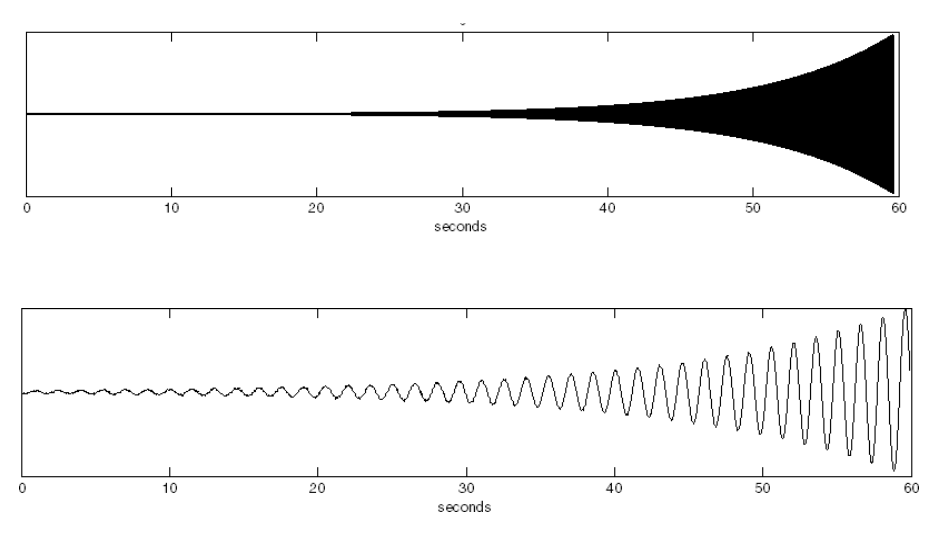
\includegraphics[width=0.95\linewidth]{figs/quint.png}
  %\caption{Above: Normal waveform, below: quintessence waveform, source: \citep{Loviscach2011}}
  %\label{fig:quint}
%\end{figure}

\citet{Gohlke2010} proposed five novel ideas on how to improve multi-track DAW displays, including techniques for
saving screen space by overlaying and stacking waveforms. One of these proposals was for a lens-like view, which
magnified the area of the waveform around the current playhead position. This allowed users to simultaneously view the
waveform at two different scales -- an overview of the audio waveform and a detailed local view. This concept has the
potential to display frequency information in regions of interest, and help make more precise audio edits without
adjusting the overall zoom level.

%waveform tracks can vertically overlap by 25\% without dramatically affecting display quality
%waveforms are mostly symmetrical, so by discarding one half the overlap can be increased to 50\%
%stack graph for contribution of each track to perceived loudness

\paragraph{Colour}
The use of colour is a simple and effective way of adding additional information to a waveform.  However, many DAWs use
waveform colour to distinguish or label audio clips, and most others have monochromatic waveforms.  Previous research
has experimented with mapping semantic audio features to colour, using either pseudocolour or false colour.

\textit{Pseudocolour} is a method of mapping a scalar value to a colour gradient \citep{Moreland2009}, an example of
which is thermal imaging cameras.  Colour gradients are composed of at least two colours (e.g. blue to red) or a
spectrum of colours (e.g. a rainbow).  Pseudocolour allows values to be mapped to colours that might be perceptually
relevant (e.g. green/red for good/bad).  It can emphasize small variations between values by using a full spectrum,
pick out high/low values using non-linear gradients, or categorize values using stepped gradients.  However, as
pseudocolour can only represent one dimension, it does not make full use of the available colour space.

\textit{False colour} is the mapping of multiple values to the dimensions of a colour space. Commonly, three values are
mapped to red/green/blue (RGB) colour space. Other colour spaces can be used, such as hue, saturation, value (HSV),
which better matches human perception of colour. Hue means colour on a rainbow, saturation means lack of grayness, and
value means brightness. The advantage of this method is that it can make full use of the available colours.  On the
other hand, it can be challenging to select three values and map them to colour in a way that is perceptually relevant
and understandable.

\citet{Rice2005} presented \textit{Comparisonics}, which uses pseudocolour to map the frequency content of an audio
signal to a colour spectrum.  Comparisonics was designed for identifying timbrally distinct sounds and they claim that,
with training, it can be used to identify certain sound effects.  Their technique maps low/mid/high frequencies to
blue/green/red colours, respectively, using an unpublished algorithm.  Comparisonics has since been integrated into the
\textit{Scratch LIVE} DJ software from Serato Audio Research, where it was used to distinguish between different drum
noises, such as bass kicks, snares and high-hats.

A very similar system was implemented in the audio clip sharing website \textit{Freesound} \citep{Akkermans2011} to
help users quickly find and compare sound effects and music clips.  They used pseudocolour to map the ``spectral
centroid'' of the audio to a colour gradient.  Spectral centroid is the weighted mean of the frequencies of a signal
\citep[p. 10]{Smaragdis2009}, so a low value indicates the presence of mostly low-frequency sound and vice-versa.

\citet{Loviscach2011a} used pseudocolour to enhance the navigation of speech. The ``zero-crossing rate'' of the audio
was mapped to a red/green/blue colour spectrum to help distinguish between different phonemes (e.g. ``oo'' or ``s'').
The zero-crossing rate is the frequency with which an audio signal switches between a positive and negative value
\citep[p. 37]{Zhang2010}, which is a crude measure of the primary frequency of the audio.

\citet{Tzanetakis2000} used false colour to create a visualisation technique known as \textit{Timbregrams}. Their aim
was to ``use color perception and the pattern recognition capabilities of the human visual system to depict timbral and
temporal information''.  Their implementation extracted a large vector of common audio features, then used principal
component analysis to reduce the size of the vector whilst retaining 80\% of the variance in their data.  They mapped
the first three principal components of the feature to RGB or HSV colour space.  They found that the RGB colour space
was more uniform and aesthetically pleasing, but that the HSV colour space had better contrast at segmentation
boundaries. When using RGB, speech, classical music and rock could easily be distinguished as they appeared as light
green, dark blue and dark green, respectively. Tibregrams were later used to colour a waveform in a basic audio editor
\citep[p. 253]{Tzanetakis2001}.

\citet{Mason2007} used false colour to assist radio listeners in navigating recently-broadcast material. They mapped
three empirically-chosen audio features to RGB colour space. The authors reported that the system was successful at
indicating the location of music within speech content, and highlighting low-bandwidth material such as phone calls.
The authors proposed that the system could be also be applied to other applications such as segmentation of radio
programmes for re-editing into podcasts.

%\begin{figure}[p]
%\centering
%\begin{subfigure}{\textwidth}
  %\centering
  %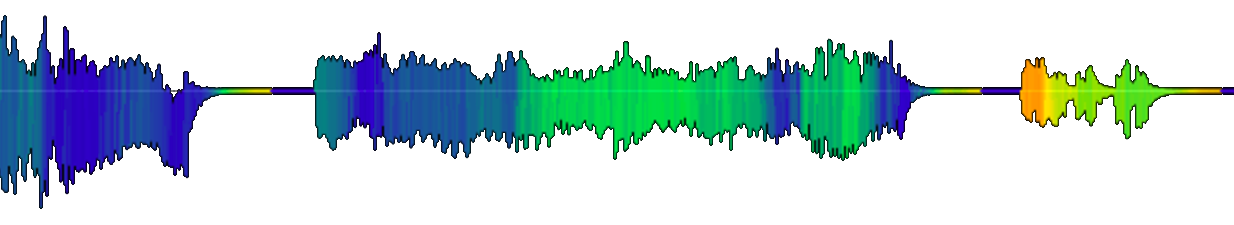
\includegraphics[width=\linewidth]{figs/freesound2.png}
  %\caption{Freesound (\url{freesound.com})}
  %\label{fig:freesound}
%\end{subfigure}\\%
%\begin{subfigure}{\textwidth}
  %\centering
  %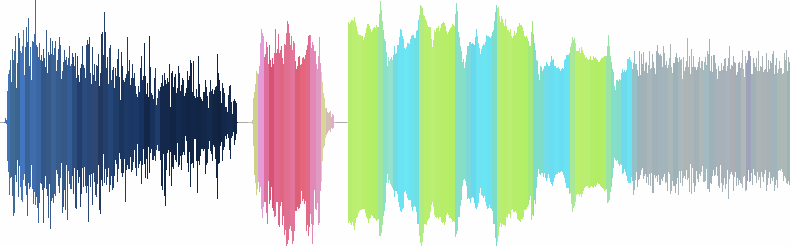
\includegraphics[width=\linewidth]{figs/rice.png}
  %\caption{Comparisonics \citep{Rice2005}}
  %\label{fig:rice}
%\end{subfigure}
%\caption{Examples of pseudocolour (\ref{fig:freesound}) and false colour
  %(\ref{fig:rice}) applied to colourising an audio waveform}
%\label{fig:colourvis}
%\end{figure}

%False colour has also been used for navigating and summarizing extremely long recordings. \citet{Towsey2014} mapped
%three spectral features to RGB colour for visualizing almost a year of environmental recording.
%Figure~\ref{fig:towsey} shows the recordings from March until October, with each line representing one day.  The
%visualization reveals the change in time of the dawn and evening choruses throughout the year, amongst other things.

%\begin{figure}[p]
  %\centering
  %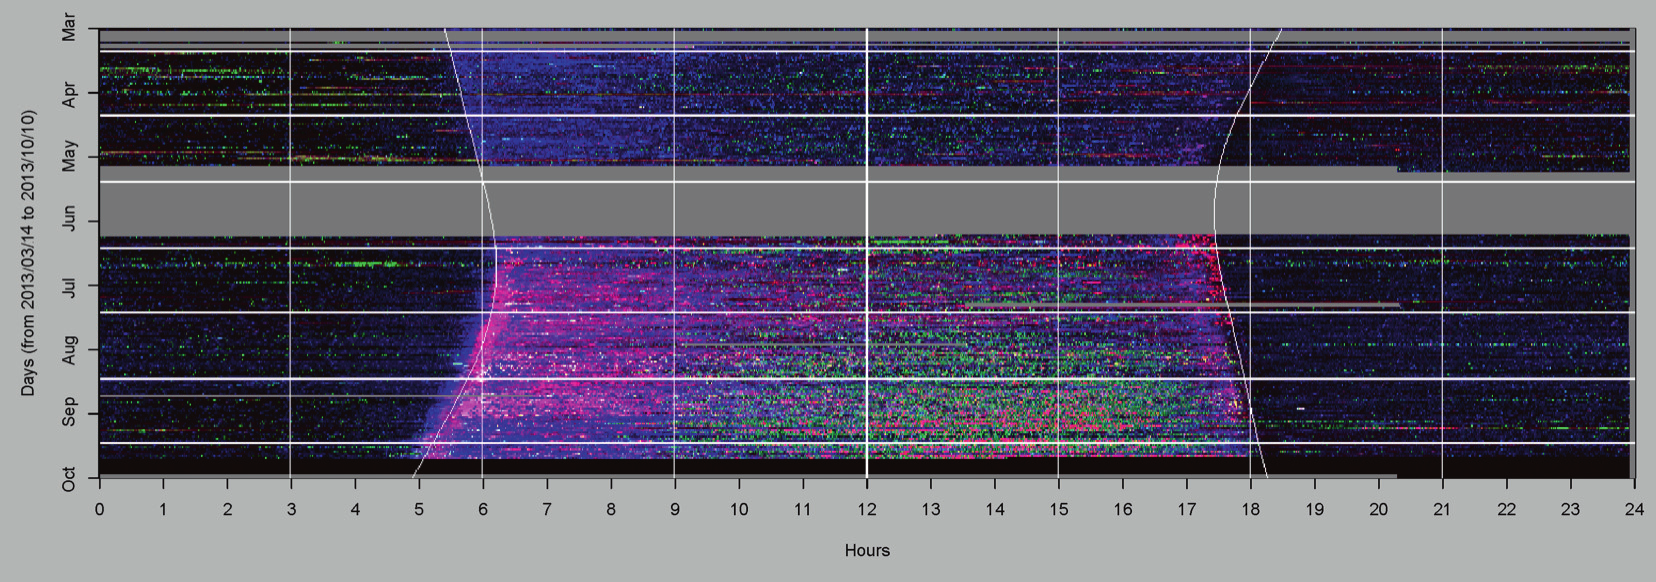
\includegraphics[width=0.95\linewidth]{figs/towsey.png}
  %\caption{False colour visualization of environmental recordings, with each line representing one day. Missing data is
    %shown in grey.
    %\citep{Towsey2014}}
  %\label{fig:towsey}
%\end{figure}

\subsubsection{Spectrograms}

Spectrograms display the amplitude of audio frequency over time. Unlike waveforms, the frequency information is visible
at all zoom levels, which makes them much more robust. They display so much information that, with sufficient training,
it is possible to read speech using a spectrogram \citep{Zue1979,Zue1986}.  However, despite these advantages, audio
waveforms are much more widely used than spectrograms in audio production.

%\citet{Gohlke2010} proposed a
%thresholded spectrogram overlaid with different colours for each track to minimuse spectrotemporal overlap and masking

\citet{Lin2012} introduced a method of filtering spectrograms to visually emphasize non-speech events in long audio
recordings. The filtering was done using an ``image saliency algorithm'' that detected differences in the intensity and
orientation of the spectrogram image. This \textit{saliency-maximized spectrogram} was integrated into an audio
navigation interface called \textit{Timeliner} \citep{Goudeseune2012}, which displayed the spectrogram alongside a
waveform. \citet{Lin2013} describes an evaluation in which 12 novice participants used Timeliner to find sound effects
hidden in meeting room recordings using both saliency-maximized and normal spectrograms. The results show that
saliency-maximized spectrograms significantly outperformed normal spectograms.
Filtering spectrograms shows promise as a way of detecting unusual events, however it is unclear how useful this sort
of application would be in the context of radio production.
%A user study of Timeliner for audio event detection \citep{Hasegawa-Johnson2011} Uses false colour to map min, mean
%and max values to the HSV colour space

%\begin{figure}[ht]
  %\centering
  %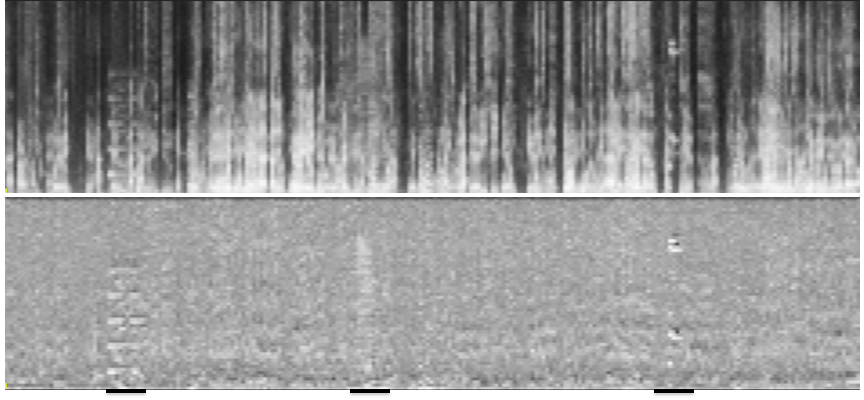
\includegraphics[width=0.95\linewidth]{figs/spectrogram-salience.png}
  %\caption{Top: A normal spectrogram; Bottom: A salience-maximised spectrogram with target events marked using black
    %underlines}
  %\label{fig:timeliner}
%\end{figure}


% Could use image synthesis \citep{Levkowitz1991}

\subsection{Segmentation}

Waveforms and spectrograms provide a direct mapping of sound to vision, which is then interpreted by the user. The
benefit of this approach is that it can be used for a wide variety of tasks with any type of content.  The downside is
that the user must learn how to read these visualizations, and view them at an appropriate scale.

With many audio recordings, the content can be divided into logical groupings that could help the user navigate the
recording. For example, a ``magazine-style'' radio programme is made up of several pieces on different topics. Being
able to view what those topics were, and where they occured in the programme, would assist listeners in navigating to
a topic of interest.

Semantic audio analysis techniques have been widely used to classify and segment audio into a range of logical
categories. These are often combined with data visualization techniques \citep{Aigner2011} to create novel user
interfaces that aid the navigation and editing of audio content.

We have divided these segmentation techniques into two broad categories: classification, where audio is segmented by
the character of the audio (speech, music etc.), and topic summarization, where the audio is segmented by its content.

\subsubsection{Classification}

Audio can be divided into human-readable segments using semantic audio analysis techniques.  Semantic audio analysis
typically operates in two main steps: dividing an audio file into sematically meaningful segments, then grouping these
segments into semantically meaningful categories \citep{Lu2009,Zhang2010}. These categories can be chosen to match the
application being targeted. For example, a radio broadcast might be divided into speech, music, speech mixed with music
and applause.

This semantic audio segmentation has applications to audio editing \cite{Avdelidis2007}.

\paragraph{Speech/music discrimination}
Speech-music discrimination (SMD) is the task of segmenting an audio recording and labelling those segments as either
speech or music.
Previous research into automated SMD has often targeted recordings of radio broadcasts
\citep{Goodwin2004,Wieser2014,Saunders1996,Pikrakis2008,Pikrakis2006a}.
%Clustering is a task in which comes naturally to humans, but machines often struggle with.




\paragraph{Speaker diarization and identification}
\textit{Speaker diarization} is the task of segmenting a speech recording according to speaker identity, which is used
to answer the question ``who spoke when?'' \citep{AngueraMiro2012}. Segments are given a unique label for each speaker,
but the identity of the speakers is unknown.  \textit{Speaker identification} is the task of identifying the person who
is speaking based on the sound of their voice.

\citet{Raimond2014} introduced the \textit{BBC World Service Archive prototype}, which was an interface that used
automatic keyword tagging and crowd-sourcing to support the search and discovery of a large radio archive.
The interface used speaker diarization and speaker identification to help users navigate within individual radio
programmes. Figure~\ref{fig:bg-world-service-archive} shows an example of a radio programme that has been segmented
into five named speakers.

\begin{figure}[ht]
  \centering
  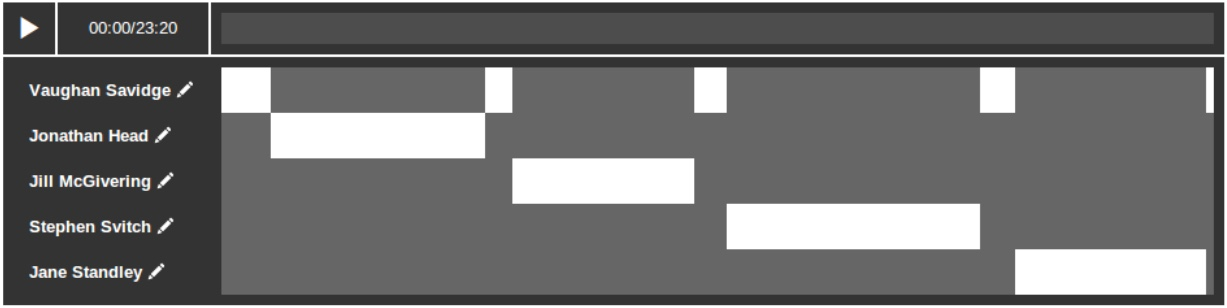
\includegraphics[width=0.8\linewidth]{figs/world-service-archive.jpg}
  \caption{Speaker diarization and identification interface in the BBC World Service Archive prototype, from
  \citet{Raimond2014}}
  \label{fig:bg-world-service-archive}
\end{figure}

%Speaker identification with crowd-sourcing achieved 85\% precision and a 43\% recall

which used speaker diarization and
identification to facilitate navigation of radio programmes. The prototype relied on crowd-sourcing to add the speaker
names, which then populated a central database of speaker identities.

Segmentation algorithms often use a threshold value to configure their sensitivity. In the case of speaker diarization,
a low threshold would increase the recall and reduce the precision. For example, more speaker turns would be detected,
but some may be incorrect.  This threshold is often set to minimise a cost function, which balances the precision and
recall.  \citet{Foote1998} describes a video browser prototype that allowed the user to control this threshold value,
using a slider in the user interface. Their prototype identified speaker turns, but did not attempt to match the
identities of the speakers.



% TOPIC SEGMENTATION
\subsubsection{Topic summarization}

Topic summarization has previously been used to assist the discovery and search of media archives \citep{Raimond2014,
Kim2003}. However, the same techniques can also be applied to aiding the navigation of audio files using segmentation.

% can use text summarization
Text summarization review paper \citep{Lloret2012}

% video digests
Video digests divide video recordings into chapters, sections and summaries.
\citet{Pavel2014} describes an interface for writing and editing video digests

% segmentation with keywords 
\citet{Abdulhamid2013,Abdulhamid2013a} introduced \textit{SpEx}, which is an interface designed to help students
navigate lecture recordings.

World service archive \citep{Raimond2014} topic extraction


% OTHER

% repeated bits
Similarity matrix can be used to discover and display repeated regions of audio \citep[p. 6]{Cooper2006}

% text
Text segmentation \citep{Choi2000}

% (below not relevant)
%Evaluation of SpeechBot for searching radio archives \citep{Kim2003}


\subsection{Text}\label{sec:background-transcripts}

% transcripts can increase the navigation speed


% two types: manually written (perfect, but expensive and slow) or automatic (erroneous, but fast and cheap)
% comparison?
Automatic speech recognition \citep{Junqua1995}, known as ``ASR'', can be used to convert speech to text.  ASR is
quicker and cheaper than manual transcription.  ASR also produces accurate timestamps for each word, which can be used
to precisely navigate and edit the audio, but word-level timestamps can also be added to manually-written transcripts
using speech alignment \citep{Griggs2007,Bohac2013}.  ASR transcripts don't include letter capitalization or
punctuation, but this can be estimated and added using post-processing.

Despite advances in the field \citep{Lee1999a}, ASR produces erroneous transcripts.  \citet{Bell2015} conducted an
evaluation of ASR systems on television programmes of various genres. Each system was judged by the proportion of
incorrect words, known as the ``word error rate'' (WER).  The mean average WER of the systems tested was 23.7\%,
however the variance across the programmes was high, with the WER varying from 10-–41\% across the 16 programmes.
Erroneous transcripts reduce listener comprehension \citep{Stark2000,Vemuri2004} and increase the time it takes to
search audio content \citep{Ranjan2006} and correct errors \citep{Burke2006}.  However, despite these errors, ASR
transcripts provide a highly effective tool for browsing audio content as users can visually scan the text to focus on
regions of interest, known as ``strategic fixation'' \citep{Whittaker2007}.

%\citet{Vemuri2004} conducted a user study of 34 participants and measured their comprehension of short audio clips when
%presented with both perfect and auto-generated transcripts.  The results show that subject comprehension of audio
%presented with a perfect transcript (C1) was found to be better than an automatically-generated transcript.
%completely wrong transcripts aren't worse than no transcript

%\citet{Ranjan2006} studied the performance of 13 participants in an audio search task with varying levels of
%transcript quality. The results showed that the mean search time descreased as the transcript quality increased.

%\citet{Burke2006} found that higher quality transcripts required users to listen less to complete a correction task.

%Automatic speech recognition technology makes it possible to extract partially accurate transcripts of speech
%recordings.  A number of researchers have experimented with using these transcripts to enhance interfaces for
%interacting with audio content.
%\subsection{Navigation}

% navigation with transcripts

\subsubsection{Transcript navigation}
Transcripts have previously been used by several systems as an interface for improving the navigation of speech-based
content such as news reports and voicemail messages. 
One of the first such systems was \textit{NewsTime} from \citet{Horner1993}, which used transcripts to aid the
navigation of audio news stories.  For television news, closed captioning was aligned the audio to provide an accurate
transcript with word timings.  NewsTime included several additional features including searching by keyword, segmenting
the transcript by story and speaker, jumping to the next or previous speaker/story, and categorizing stories into one
of seven common topics. There were no reported user studies of NewsTime.

\textit{SCAN} \citep{Whittaker1999} was an interface designed to support retrieval from speech archives. It used ASR transcripts
to allow users to search for keywords and visually search the recording by reading the transcript.  In a user study of
12 participants, the transcript was found to support navigation by reducing the listening time needed to complete
information retrival tasks. Participants rated the transcript as easier and more useful with the transcript than
without.  SCAN was further developed into \textit{SCANMail} \citep{Whittaker2002}, an interface designed for interacting with
voicemail.  It added a number of features including paragraph segmentation and the ability to seek to a point in the
audio recording by clicking on a word in the transcript. The results of a user study of eight expert users showed that
the transcript display enabled users to visually scan the content of recordings to quickly extract information and
judge which parts were relevant, without having to play the audio.
%SCANMail did not include editing capabilities

\subsubsection{Semantic speech editing}
In addition to supporting the navigation of speech recordings, transcripts have also been used as a method of editing
speech content. The first of these was the `Large Interactive Display System Wave Speech Editor', or
\textit{LIDSWSEdit}, from \citet{Apperley2002}, which used ASR transcripts to allow users to navigate and edit lecture
recordings.  Any edits made to the transcript were correspondingly applied to the underlying audio recording, known as
``semantic speech editing''. Users could re-arrange sentences and words by selecting the text, then using a
drag-and-drop action.  Alternatively, speech could be removed by selecting text then clicking a button to either delete
the selected text, or everything except the selected text.  LIDSWSEdit was further developed into the
`TRanscription-based Audio EDitor', or \textit{TRAED} \citep{Masoodian2006}.  TRAED used the same editing actions as
LIDSWSEdit, but rather than displaying the text and audio waveform separately, it displayed the waveform in-line with
the text. Individual words were indicated by drawing boxes around the waveform and word. The boundary between each word
pair could be adjusted by dragging the boundary edge.  We could not find any user studies of LIDSWSEdit or TRAED.

\citet{Whittaker2004} created an interface for editing voicemail messages using ASR transcripts.  Users could
cut-and-paste parts that they wanted and delete other parts.  The system was evaluated in a formal study of 16
voicemail users, which found that semantic editing was faster and as accurate as editing with a waveform-based
interface. Crucially, this was true even though the transcripts had an average word error rate of 28\%. This
demonstrates that semantic editing is beneficial even when using erroneous transcripts.

\citet{Rubin2013,Rubin2015} presented a novel interface for creating ``audio stories'' that, similarly to radio
programmes, combine speech and music.  The interface used an editable transcript with two columns, one for each of a
pair of speakers.  It allowed the user to cut, copy, paste and delete the audio using the text. It also highlighted
repeated words, similar sentences, ``umm''s, breaths and pauses in the transcript. The transcripts were generated using
a crowd-sourcing service with speech alignment software that also detected breaths.  The system also included
additional functionality for finding and adding music tracks, and for varying the length of music using automatic
looping. The system was evaluated through a short informal study of four participants where the editing capabilities
received positive feedback. No follow-up studies have been reported since.

\citet{Sivaraman2016} created a semantic editing system for asynchronous voice-based discussions, where users could
quickly edit their speech recording before sending it to the recipient.  Their system used near-live automatic
transcription and detected pauses in the speech. Their interface allowed users to delete selected words/pauses, insert
additional pauses and fix incorrect words.  In a formal qualitative study of their system with nine users, they found
that text-based editing was considered good enough to replace waveform editing, and to be more accessible. They
observed that most users only used the system to make fine-grained edits, instead of editing large chunks.  Users said
that the transcript also allowed them to quickly review all the points that were made, and that the errors in the
transcript weren't a heavy distraction. A quantiative study of 28 students and teachers found that
including editing functionality resulted in the students reporting lower levels of mental task load, effort and
temporal demand.

\citet{Yoon2014} created a collaborative tablet-based document annotation system called \textit{RichReview}, which
offered users three modalities in which to annotate documents - freeform inking, voice recording and deictic gestures
(i.e. pointing to areas of interest). The voice recordings were displayed using a waveform, overlaid with an ASR
transcript of the speech.  Users could trim or tidy the voice recordings by drawing a line through words or pauses to
remove them.  The system was evaluated using a qualitative study of 12 students which found that the editing features
were considered easy to use and efficient for removing ``umm''s and long pauses.  However many participants reported
that the transcripts were not accurate enough to use without having to listen to the audio.
%RichReview was later deployed as a web applet on the online education platform edX \citep{Yoon2015a}.
\citet{Yoon2016} describes two deployment studies that used a similar system called RichReview\textsuperscript{++}, but
this did not include any semantic editing functionality.

\subsubsection{Video editing}
Semantic speech editing has also been used to support video editing.  \textit{SILVER} \citep{Casares2002, Long2003} was
a video editor that aligned words from closed captions to the video.  Gaps, errors and edits were displayed in the
transcript using special characters.  The video could be edited by deleting text in the transcript.  SILVER was
evaluated in an informal study with seven students, but the study did not report any results about the transcript-based
editing feature.

Hyperaudio Pad is an open-source audio and video editor, first proposed by \citet{Boas2011}, and now available online
as a free service \citep{Hyperaudio2016}. This is a web-based interface that allows users to navigate and edit online
media using transcripts. The transcripts are generated from subtitles by using speech alignment software. Editing is
done by selecting a part of the transcript and dragging it into a window to create a `clip'.  Other clips can be added
and re-ordered, and the edited version can be played and shared with others. No user studies of this system could be
found.

% video editing using perfect transcripts
When editing a video interview, you want to avoid making a cut when the person speaking is in shot, because it causes
the image to suddenly jump.  \citet{Berthouzoz2012} used image processing algorithms to create a video editor that can
help the user hide these edit points. The editor had an editable transcript window that displayed suitable edit points
and allowed the user to edit the video by selecting and deleting text. The transcripts were generated manually using an
online crowd-sourcing service, and word timings were added using speech alignment software. The system also allowed
users to easily remove `umm's or repeated words as they were explictly marked in the manual transcript. No user study
was conducted in the reported study, however positive feedback was received from nine professionals who were given a
demonstration.

\subsubsection{Pre-written scripts}
The systems so far have only considered transcripts that have been generated from the speech itself. However, sometimes
speech is recorded based on a pre-written script, or from notes.  Avid released a feature for their Media Composer
video editing software in 2007 called \textit{ScriptSync} \citep{Avid2011}.  This feature aligns a user-supplied
transcript to a video recording by placing a marker in the video for each line of the transcript \citep{Griggs2007},
allowing users to jump to a particular line, or see which line in the transcript corresponds to the current point in
the video.  A second version of ScriptSync was launched in February 2017 \citep{Avid2017} which added script correction
and collaborative note-taking.
%We did not find any reported user studies of ScriptSync.

\citet{Shin2016} created a system called \textit{Voice Script} that supports an integrated workflow for writing
scripts, and recording/editing audio. An informal study with four amateur participants found that it could support
various workflows including multiple iterations. It included a `master script' layout which was used to bring together
different recordings,  and that was found to work well.  A second study of four amateur participants directly compared
the system to that of \citet{Rubin2013}, which found that participants were able to complete an audio production task
25\% faster using the Voice Script system.  This study demonstrates that for workflows that involve pre-written
scripts, there is potential to improve the audio editing by using an integrated writing and editing system.

\textit{QuickCut} from \citet{Truong2016} was an interface designed to help producers edit a narrated video from a
pre-written script, voiceover audio and raw video footage.  Producers could label their video footage using their
voice, which was manually transcribed using a crowd-sourced online service. Speech alignment was used to align the
script to the voiceover audio.  Selecting text in the script also selected the corresponding segment in the voiceover
audio, and displayed video clips that were labelled with similar words. After selecting an appropriate clip, it could
be added to the timeline using drag-and-drop to associate it with a position in the script.  The completed timeline
could then be exported as and ``edit decision list'' (EDL) for use in professional video editing software.  QuickCut
was evaluated by the researchers themselves and one professional filmmaker, who were able to use the system to produce
videos in a fraction of the time normally needed.  Voice-based logging makes sense for logging video footage as it is
easy to watch and talk at the same time. However, for speech content it would be difficult to talk and listen
simultaneously.  The ability to export edits to professional software allows for a smooth continuation of the
production workflow.

%ellipses were used to indicate pauses.
%three constraints - alignment, alternative, ordered

% CORRECTION

\subsubsection{Transcript correction}
SILVER \citep{Casares2002, Long2003} 

\citep{Masoodian2006} included correction by selecting a word and typing a replacement. New spaces created a new word,
dividing the time in half.

\citet{Burke2006} added correction functionality to the SCANMail interface by allowing users to either select a
replacement word from a drop-down menu, or select multiple words and type over them. A user study of 16 participants
correcting voicemail messages showed that the menu interface required much less listening than typing.

\citet{Liang2014} showed that once an incorrect word is identified, in 30\% of cases the correct word can
automatically be inferred using $n$-grams and acoustic features.

Normally, correction is a post-production process that can take up valuable time, although as \citet{Wald2007} shows,
real-time correction of speech is feasible.

\citep{Suhm2001}

%TypeTalker - editing spoken comments \citep{Arawjo2017}
\textit{TypeTalker} from \citet{Arawjo2017} was an interface for editing synthesized speech comments using ASR
transcripts. The speech was synthesized from recordings of the user's comments, which was done to reduce their
self-consciousness. As well as being able to remove unwanted speech, the use of speech synthesis meant that new speech
could be inserted and words could be changed.

%Colour, size and orientation guide visual attention for visual search \citep{Wolfe2004}

% confidence shading
\subsubsection{Confidence shading}
In addition to producing a transcript, many automatic speech recognition systems return a confidence score for each
transcibed word, indicating how sure the system is that the word is correct. ``Confidence shading'' is a technique for
displaying this score by colouring words with a low confidence score in a lighter shade.
Confidence shading has been used in an attempt to make mistakes easier to locate, and transcripts easier to read.
%It is hypothesised that confidence shading makes it easier to identify incorrect words for the purposes of correction,
%and increases the comprehension of the text because the lighter shade makes mistakes less apparent.
Confidence scores may themselves be incorrect by indicating false positives (when a correct word is marked as
incorrect), or false negatives (when an incorrect word is missed). The balance between the two is controlled using the
threshold value between 0 and 1. As \citet{Feng2004} demonstrates, a higher value reduces false positives and increases
false negatives, while a lower value increases false positives and reduces false negatives.

\citet{Suhm2001} conducted a user study of 15 participants who corrected an ASR transcript with and without confidence
shading (in this case, highlighting). The results showed that correction with confidence shading took slightly longer
than without, although this was not statistically significant.  Conversely, \citet{Burke2006} reported that users find
confidence shading helpful. 16 participants performed a transcript correction task with confidence shading and overall
they agreed that shading was helpful for identifying mistakes.  One notable difference between these studies is that
\citet{Suhm2001} optimised their confidence threshold to minimise the overall accuracy of the confidence shading, whilst
\citet{Burke2006} increased the threshold to treat false negatives more seriously.

\citet{Vemuri2004} studied whether confidence shading improved comprehension of the transcript. They conducted a user
study of 34 participants and measured the comprehension of short audio clips when using ASR
transcripts with and without confidence shading. Although the results indicated better comprehension with confidence
shading, there was no statistically significant difference.

\subsubsection{Keyword extraction}

Keyword extraction \citep{Matsuo2004}

Keywords used by \citet{Loviscach2011a} as part of his nimble video editor

% keyphrases from speech, using ASR, poor quality
Extracting keyphrases \citep{Inkpen2004}


%TODO other applications
%Coding of video interviews \cite{Chandrasegaran2017}

%VisScribe - interactive transcript interface and speaker activity for coding design sessions \cite{Chandrasegaran2017}

%Personal device for recording and navigating notes using keywords \citep{Tucker2003}


\subsection{Audio user interfaces}

The previous work we have considered so far have used rich visualizations to display complex representations of
transcripts, speakers, structure and summarizations. Visual presentation of audio content makes it easier for users to
search and skim the information, but it is difficult, if not impossible, for humans to fully comprehend sound using
visual means. Listening is the natural way for humans to consume audio content, but the time required to listen can
make it a lengthy and inefficient process.

Audio processing and user interface design can be used to increase the speed and precision with which users can listen
to and interact with audio. Previous research has demonstrated this using a variety of techniques, including processing
the audio to improve the comprehension of speech at higher playback rates, re-designing audio scrolling interfaces for
better control of playback, exploiting the ``cocktail party effect'' by playing multiple audio streams simultaneously
to search for specific moments in recordings, and using audio spatialization to allow for spatial navigation of audio.
We discuss each of these techniques below.

\subsubsection{Time compression}

% problem description
Listening to long audio recordings of speech can be time-consuming. A simple way to reduce the listening time is to
increase the rate of playback.  However, this increase in speed causes an upward shift in the pitch of the sound, which
degrades the speech and makes voices sound like cartoon characters.  The increased speed with which the content is
presented also makes it difficult for listeners to process the information fast enough.

These limitations negatively affect the intelligibility and comprehension of the speech.  In this context,
\textit{intelligibility} refers to the ability to identify words, and can be measured by the accuracy with which a
specific word is recalled. \textit{Comprehension} refers to the ability to understand the content of the material,
measured by the number of correctly answered questions about the subject matter.

%By carefully selecting which words to listen to, speech
%can remain intelligible at up to 10-times normal speed \citep[p.~7]{Arons1997}.
%TODO better citation needed

% difference between time compression and speech skimming
There are several approaches for reducing the time required to listen to a recording while being able to extract
critical information, which can be divided into two categories. \textit{Speed-up} techniques aim to increase the speed
of playback without affecting the pitch of the speech, and \textit{excision} techniques aim to remove parts of the
speech in a way that minimises the reduction in comprehension.

% speed-up vs excision
\citet{Tucker2006} performed a user study that compared two different excision techniques and a speed-up technique,
using both 5-min and 30-min audio recordings.  Participants ranked a list of utterances to match what they heard,
which was compared to a reference response to produce a score for comprehension. This score was normalised by the
listening time to measure ``comprehension efficiency''.  The results showed that for short recordings, excision
outperformed speed-up, but that they performed similarly for long recordings. However, participants reported that they
prefered excision and were less likely to switch to normal-speed playback when using it.

%time compression and speech skimming.
%\textit{Time compression} refers to a set of sampling techniques that are used to reduce the length of the audio by
%skipping or over-lapping audio frames.  \textit{Speech skimming} exploits the natural boundaries and acoustic
%properties of speech to structure the audio content based on salience. This can be determined based on the location and
%frequency of natural pauses, the emphasis of the voice (usually determined by pitch), speaker diarization and the
%content of the speech.

% time compression (sampling techniques)
% - shortening/removing pauses
% - isochronous sampling (regularly skipping frames)
% - SOLA (overlapping frames)
% - dichotic sampling
% - backward sampling
%
% skimming (structuring the audio by segmenting based on saliency, then skipping)
%   - pauses
%   - pitch-based emphasis
%   - content-based
%   - speaker diarization

% excision techniques
% isochronous sampling, shortening/removing pauses
The simplest excision technique is to remove frames of audio at regular intervals, known as ``isochronous sampling''.
However, this approach does not discriminate between valuable and redundant information. It also fails to take into
account speech boundaries, so may cut the audio mid-way through a word. Shortening or removing pauses between words is
a simple and effective approach that reduces the length of the audio whilst retaining all of the information and
respecting speech boundaries. However, once all of the pauses have been removed, other techniques must be used to
further compress the speech.

% emphasis detection
%Early work by \citet{Heiman1986} showed that double-speed playback removes virtually all redundant information, so when
%playing back at higher speeds, information is lost. To avoid losing important information, some excision algorithms
%attempt to segment the recording according to the relevance of the content. The audio is then compressed by only
%playing only the beginning of each segment.

Many exicision algorithms operate by segmenting the audio at points of increased saliency, then playing only the
beginning of each segment before moving onto the next. The saliency can be determined by measuring pause length, pitch,
speaker turns and the content.  Long pauses in speech often signal a new sentence, thought or topic, which can be an
indication of importance. The pitch of the voice tends to increase in range when introducing a new topic, which can be
used as a measure of emphasis.  Speaker diarization techniques \citep{AngueraMiro2012} can be used to detect changes in
speaker, which can be a cue for changes in topic. Transcripts of the speech have also been used with summarization
techniques to determine the most salient parts of the speech, using both ASR transcrips
\citep{Hori2003} or manually-written transcripts \citep{Tucker2006}.

\textit{SpeechSkimmer} by \citet{Arons1997} combined three excision techniques into a single time compression interface
by switching between them for different rates of playback. He used pause shortening and removal for modest speed
increases, followed by pause-based segmentation for faster playback. For the fastest playback rate, he used segmentaton
resulting from a pitch-based emphasis detection algorithm. He evaluated the system through a qualitative study of 12
participants which compared two systems that used different algorithms for the fastest playback rate -- one using
pitch-based emphasis segmentation and the other using isochronous sampling. The participants reported that pitch-based
emphasis was effective at extracting interesting points, and performed better than excision using isochronous sampling.

There are limits to how far time compression can be used to increase playback speed.  For example, speed-up techniques
are only intelligible up to a maxiumum of around 2x to 2.6x real-time
\citep{Vemuri2004,Tucker2006,Ranjan2006,Arons1997}.  However, transcripts can be used in combination with time
compression to increased this maximum rate.  \citet{Vemuri2004} conducted a user study of 34 participants and measured
their comprehension of short audio clips at different rates of playback using speed-up. The mean self-reported maximum
playback rate was 2.6x real-time for listening only. The addition of an ASR transcript increased
this to 2.8x, and an accurate transcript increased this further to 3.0x.  Several systems have successfully combined
transcripts and time-compressed playback \citep{Whittaker2002}.
%TODO More system examples

% PROS
% - listening to audio, which is more natural and rich than text
% - can halve the time needed to listen, up to a third the time with perfect transcript

% CONS
% - increases cognitive load, more tiring for listeners
% - excision is preferred, okay for aiding memory but probably not suitable for first-time listening
%   - might miss something out
%   - harder to judge suitability of audio (e.g. prosody affected by pause shortening/removed
%   - algorithms filtering content could inadvertenty affect creativity/balance

\subsubsection{Simultaneous playback}

The \textit{cocktail party effect} is ``the ability to focus one's listening attention on a single talker among a
cacophony of conversations and background noise'' \citep{Arons1992}.  This effect can be exploited to help listeners
find a particular piece of audio in a recording by playing different parts of that recording simultaneously. To help
listeners separate the sounds, previous work has experimented with using headphones to play different sounds in each
ear, or using binaural audio to spatially separate the sounds. 

\textit{AudioStreamer} from \citet{Schmandt1995} used binaural spatialization techniques to play three simulataneous
audio streams of broadcast news around a listener's head. The system tracked the movement of the listener's head to
boost the level of the stream they were facing as they turned.  In addition, they used pause-based segmentation and
speaker diarization to alert the listener to new stories using a short bleep sound. No user studies of AudioStreamer
were conducted.

\textit{Dynamic Soundscape} from \citet{Kobayashi1997} also used spatialization to help users navigate audio files by
mapping the sound to fixed positions a virtual soundscape. The system was designed to take advantage of human abilities
for simultaneous listening and memorising location. Users would start by listening to a virtual ``speaker'' that played
the audio while slowly orbiting their head in a clockwise direction. Audio could be replayed by pointing their hand 
at the location where it was originally heard, which would create a second speaker that played from that position.
Similarly, users could skip ahead by pointing to a position ahead of the original source.  Speakers could be grabbed
and moved, and an audible ``cursor'' allowed users to hear where they were pointing.  Through informal feedback, users
suggested that they could use their spatial memory to navigate the audio. Based on their observations, the authors
suggested that the system could help with transfer to long-term memory.

\citet{Ranjan2006} attempted to reduce the time needed to search an audio recording by using \textit{dichotic
presentation}, where different sounds are played into each ear.  In their system, the left ear played from the
beginning of the recording while the right ear played from the half-way point. Through a user study of 13 participants,
they tested the effectiveness of this approach for a search task. The results showed that dichotic presentation reduces
the overall search time, particularly when the answer is in the second half of the recording. However, the overall time
reduction was only around 20\%.  Dichotic presentation can be combined with time compression, but this creates high
cognitive load and 8 of the 13 participants reported it to be ``very demanding''.

%50x video playback with audio skimming on BBC rushes \citep{Christel2008}

%Skimming and markers \citep{Dhanesha2010} for use on normal telephone

%\citet{Imai2001} proposed a speed-up algorithm for Japanese speech, with a view to using it for video editing. They
%tested the comprehensibility of their algorithm on 6 participants which indicated that speech can be comprehensible at
%up to x5 speed. They implemented their algorithm in a non-linear video editing system, but did not attempt to evaluate
%it.

%\subsubsection{Scrolling interfaces}
%Elastic Audio Slider \citep{Huerst2004}
%Position-based audio slider \citep{Huerst2006}
%MobileZoomSlider, ScrollWheel \citep{Huerst2008}
%Hardware scrolling interfaces \citep{Lee2007}
%DiMa\ss \citep{Lee2006}

%\subsubsection{Haptic interfaces}
%Haptics
%\citep{Metatla2016}

%\subsubsection{Mix audio and text}
%Quixotic: Audio recorder with word processing interaction \citep{Milota2015}

\clearpage
\section{Research scope and methodology}

% - better understanding of the current tools and their performance
% - better understanding of the radio production process and which techniques could be used to improve it
% - apply one or more of these techniques and test its effect in radio production to see:
%   - whether it works
%   - what the challenges are
%   - identify missing elements for future research

Process for designing and evaluating interfaces for audio industry \citep{Dewey2014}

In previous sections, we outlined
An initial investigation of prevailing techniques revealed
Therefore, in order to achieve the full potential of 
we argue for advancements in 
and consider these advancements vital in applications like 
An underlying hypothesis for this work is that
This may be achieved by

A characteristic problem within the scope of this work is related to 
Since data collection in the studio is a difficult task in itself, we focus on
We argue that
We aim to show that

% make the most of access to producers
The author is an employee of the  Research and Development department at the BBC. This position allows him access to
producers working in BBC Radio, both physically and politically. This is unusual in academic research, where often
there is difficultly in gaining access to industry professionals and in running academic studies outline of a
laboratory. In this research, we wanted to take advantage of this position by using, where possible, the professional
resources available to the author that other researchers would not be able to access. This would allow the best
contribution to the field given the circumstances of the author's position. The direction of research during this work
was often guided by this decision.

